
% Este documento LaTeX fue diseado por profesores  del Departamento de Matemticas 
% de la Universidad de Antioqua (http://ciencias.udea.edu.co/). Usted puede modificarlo
% y personalizarlo a su gusto bajo los trminos de la licencia de documentacin libre GNU.
% http://es.wikipedia.org/w/index.php?title=Licencia_de_documentaci%C3%B3n_libre_de_GNU&oldid=15717448

\documentclass[serif,9pt]{beamer}
\setbeamertemplate{navigation symbols}{}


\usetheme{Warsaw}

%\documentclass[serif,9pt]{beamer}
%\usepackage[T1]{fontenc} % Needed for Type1 Concrete
%\usepackage[charter]{mathdesign}


%\usepackage[pdftex]{graphicx}

\usepackage[latin1]{inputenc}
\usepackage[spanish]{babel}

\beamersetuncovermixins{\opaqueness<1>{25}}{\opaqueness<2->{15}}

\begin{document}
\title[El problema de existencia y regularidad para las \ldots ]{El problema de existencia y regularidad para las ecuaciones de Navier-Stokes: uno de los siete problemas del milenio}  
\author{Nicols Bourbaki}
\institute[Departamento de Matemticas]{%
  Departamento de Matemticas\\
  Universidad de Antioquia}
\date{Copyleft \copyright{} 2008. Reproduccin permitida bajo los \\
      trminos de la licencia de documentacin libre GNU.}

\logo{
\includegraphics[scale=0.4]{logoudea}} 


\begin{frame}
\titlepage
\end{frame}

\begin{frame}\frametitle{Contenido}\tableofcontents
\end{frame} 


\section{Introduccin} 

\subsection{Qu son las ecuaciones de Navier-Stokes?}

\begin{frame}\frametitle{Qu son las ecuaciones de Navier-Stokes?} 

\begin{itemize}

\item Son un conjunto de ecuaciones en derivadas parciales no lineales  que describen el movimiento de un fluido (liquidos y gases). \pause
\bigskip

%\item Las ecuaciones de Navier-Stokes reciben su nombre de Claude-Louis Navier y George Gabriel Stokes. \pause
%\bigskip

\item Modelan una gran variedad de fenmenos fsicos complejos: \medskip
\begin{itemize}
 \item clima \pause \medskip
 \item corrientes ocenicas  \pause \medskip
 \item aerodinmica \pause \medskip
 \item movimiento de estrellas 
\end{itemize} \pause
\bigskip

\item No se conoce una frmula que resuelva las ecuaciones (solucin analtica) excepto en algunos tipos de flujos concretos.
\pause
\bigskip

\item Es necesario recurrir al anlisis numrico para determinar soluciones aproximadas.
\bigskip

\end{itemize}

\end{frame}

\subsection{Cmo surgen?}
\begin{frame}
\frametitle{Cmo surgen?} 

\begin{block}{Daniel Bernoulli (1700 - 1782)}
\begin{columns}
\column{.1\textwidth} \hspace{0.9cm}
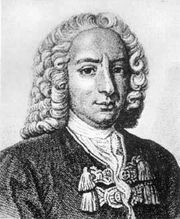
\includegraphics[width=\textwidth]{Danielbernoulli} 
\column{.8\textwidth}
Durante la primera mitad del siglo XVIII el matemtico suizo Daniel Bernoulli muestra cmo adaptar los
mtodos del clculo para analizar cmo fluyen los fluidos.
\end{columns}
\end{block}

\pause
\bigskip

\begin{block}{Leonhard Euler (1707 - 1783)}
\begin{columns}
\column{.1\textwidth} \hspace{0.9cm}
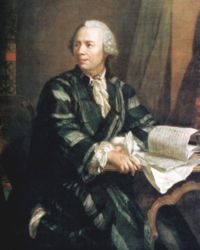
\includegraphics[width=\textwidth]{Euler} 
\column{.8\textwidth}
Basado en el trabajo de Bernoulli, Leonhard Euler formula un conjunto de ecuaciones cuyas soluciones decriben
precisamente el movimiento de un fluido hipottico no viscoso.
\end{columns}
\end{block}

\end{frame}


\begin{frame}\frametitle{ Cmo surgen?} 

\begin{block}{Claude-Louis Navier (1785 - 1836)}
\begin{columns}
\column{.1\textwidth} \hspace{0.9cm}
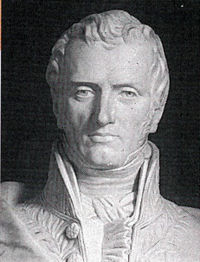
\includegraphics[width=\textwidth]{Navier} 
\column{.8\textwidth}
En 1822 Navier modifica las ecuaciones de Euler para abarcar el caso ms realista de un fluido con viscosidad.
Aunque su razonamiento matemtico fue incorrecto, obtuvo las ecuaciones correctas.
\end{columns}
\end{block}

\pause
\bigskip

\begin{block}{George Gabriel Stokes (1819 - 1903)}
\begin{columns}
\column{.1\textwidth} \hspace{0.9cm}
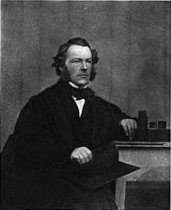
\includegraphics[width=\textwidth]{Stokes} 
\column{.8\textwidth}
En 1842 Stokes deduce por medio de un razonamiento correcto las ecuaciones que 20  aos antes Navier haba obtenido
y extendi la teora. 
\end{columns}
\end{block}

\end{frame}

\subsection{Problema matemtico}
\begin{frame}\frametitle{Problema matemtico} 

\begin{itemize}
\item Los matemticos aun \textbf{no} consiguen demostrar si para el caso en tres dimensiones
\textit{siempre} existirn soluciones (\textit{existencia}).  \pause
\bigskip

\item En caso de existir, contendrn dichas soluciones discontinuidades o singularidades (regularidad)?  \pause
\bigskip

\item El instituto Clay de Matemticas ha denominado a ste como uno de los siete \href{http://www.claymath.org/millennium/}{problemas del milenio}. \pause

\bigskip

\item El instituto Clay ofrece la suma de \textbf{un milln de dlares} a quien presente una solucin o un contraejemplo a 
este difcil problema.
\end{itemize}

\end{frame}

\begin{frame}\frametitle{Problema matemtico}

%\begin{block}{title of the bloc}
%bloc text
%\end{block}

%\begin{alertblock}{title of the bloc}
%bloc text
%\end{alertblock}

\vspace{-1cm} %Esta insturccin sube el siguiente bloque 1 cm.

\begin{exampleblock}{Anuncio del Instituto Clay de Matemticas}
\medskip
\textbf{Navier-Stokes Equation}\\ 
\medskip
Waves follow our boat as we meander across the lake, and turbulent air
currents follow our flight in a modern jet. Mathematicians and physicists
believe that an explanation for and the prediction of both the breeze and
the turbulence can be found through an understanding of solutions to the
Navier-Stokes equations. Although these equations were written down
in the 19th Century, our understanding of them remains minimal. The
challenge is to make substantial progress toward a mathematical theory
which will unlock the secrets hidden in the Navier-Stokes equations.\\ 
\medskip
\href{http://www.claymath.org/millennium/Navier-Stokes\_Equations/}{http://www.claymath.org/millennium/Navier-Stokes\_Equations/}
\end{exampleblock}

\end{frame}


\section{Descripcin del problema} 

\subsection{Las ecuaciones de Euler}
\begin{frame}\frametitle{Las ecuaciones de Euler para el movimiento de fluidos} 
\begin{itemize}
\item  Las ecuaciones de Euler gobiernan el flujo de un fluido hipottico sin viscodidad que se extiende
de manera infinita en todas las direcciones. \pause
\bigskip
\item Asumimos que cada punto $P=(x, y, z)$ en el fluido est sujeto a fuerzas que varan con el tiempo en cada 
direccin: $f_x(x,y,z,t)$, $f_y(x,y,z,t)$ y $f_z(x,y,z,t)$.\pause
\bigskip
\item El fluido experimenta una presin $p(x,y,z,t)$ en el punto $P$ al tiempo $t$. \pause
\bigskip
\item El movimiento del fluido en el punto $P$ al tiempo $t$ queda determinado por la velocidad con que
fluye en cada direccin: $u_x(x,y,z,t)$, $u_y(x,y,z,t)$ y $u_z(x,y,z,t)$. 
\end{itemize}

\end{frame}

\begin{frame}\frametitle{Las ecuaciones de Euler para el movimiento de fluidos} 
\begin{itemize}

\item  Asumimos que el fluido es \textit{incompresible}: no se puede ``comprimir'' o ``expandir'' cuando actan fuerzas
sobre ste.\pause
\bigskip

\item La \textit{incompresibilidad} se expresa matematicamente por medio de
\begin{equation}\label{incompresible}
 \frac{\partial u_x}{\partial x} + \frac{\partial u_y}{\partial y} + \frac{\partial u_z}{\partial z} = 0
\end{equation}\pause
\smallskip

\item El problema presupone que conocemos cmo es el movimiento del fluido al inicio cuando $t=0$, i.e.,  $u_x(x,y,z,0)$, $u_y(x,y,z,0)$ y $u_z(x,y,z,0)$ son conocidas (condiciones iniciales).\pause
\bigskip

\item Estas funciones iniciales deben satisfacer ciertas hiptesis de ``suavidad'' o regularidad que ms adelante en la seccin (\ref{enunciado}) precisaremos.
\end{itemize}

\end{frame}

\begin{frame}\frametitle{Las ecuaciones de Euler para el movimiento de fluidos} 
\begin{itemize}

\item  Al aplicar las leyes de Newton a cada punto $P$ del fluido y la ecuacin de la incompresibilidad \eqref{incompresible} Euler obtuvo \pause
\vspace{0.1cm}
\begin{align}
\frac{\partial u_x}{\partial t} + u_x\frac{\partial u_x}{\partial x} + u_y\frac{\partial u_x}{\partial y} + 
u_z\frac{\partial u_x}{\partial z} &= f_x(x,y,z,t) -  \frac{\partial p}{\partial x} \label{ux} \\
\frac{\partial u_y}{\partial t} + u_x\frac{\partial u_y}{\partial x} + u_y\frac{\partial u_y}{\partial y} + 
u_z\frac{\partial u_y}{\partial z} &= f_y(x,y,z,t) -  \frac{\partial p}{\partial y} \label{uy} \\
\frac{\partial u_z}{\partial t} + u_x\frac{\partial u_z}{\partial x} + u_y\frac{\partial u_z}{\partial y} + 
u_z\frac{\partial u_z}{\partial z} &= f_z(x,y,z,t) -  \frac{\partial p}{\partial z} \label{uz}
\end{align}\pause

\medskip
\item Las ecuaciones diferenciales parciales \eqref{incompresible} -- \eqref{uz} son conocidas como las \textit{ecuaciones de Euler} para el movimiento de un fluido.

\end{itemize}

\end{frame}

%\begin{figure}
%\includegraphics[scale=0.2]{convection} 
%\caption{show an example picture}
%\end{figure}

\subsection{Las Ecuaciones de Navier-Stokes}
\begin{frame}\frametitle{Las Ecuaciones de Navier-Stokes}

\begin{itemize}

\item  Navier y Stokes modifican las ecuaciones de Euler para abarcar el caso ms realista de un fluido con viscosidad.. 

\pause
\medskip

\item Introducen una constante positiva $\nu$ que mide las fuerzas de friccin en el interior del fluido.
\pause
\medskip

\item Agregan al lado derecho de las ecuciones de Euler \eqref{ux} -- \eqref{uz} una fuerza adicional (debido a la viscosidad), dada en el caso de \eqref{ux} por
\begin{equation*}
\nu \left(\frac{\partial^2 u_x}{\partial x^2} + \frac{\partial^2 u_x}{\partial y^2} + \frac{\partial^2 u_x}{\partial z^2}\right)
\end{equation*}
\pause 
\smallskip

\item Para \eqref{uy} y \eqref{uz} el trmino a agregar es el mismo pero sustituyendo a $u_x$ por $u_y$ y $u_z$ respectivamente.

\end{itemize}
\end{frame}


\begin{frame}\frametitle{Las Ecuaciones de Navier-Stokes} 
\begin{itemize}

\item  Las ecuaciones que Navier y Stokes obtienen son \pause
\medskip
%\vspace{0.1cm}
\begin{align}
\frac{\partial u_x}{\partial t} + u_x\frac{\partial u_x}{\partial x} + u_y\frac{\partial u_x}{\partial y} + 
u_z\frac{\partial u_x}{\partial z} &= \nu \left(\frac{\partial^2 u_x}{\partial x^2} + \frac{\partial^2 u_x}{\partial y^2} + \frac{\partial^2 u_x}{\partial z^2}\right) \nonumber\\ & + f_x(x,y,z,t) - \frac{\partial p}{\partial x}\label{nsux}\\  \frac{\partial u_y}{\partial t} + u_x\frac{\partial u_y}{\partial x} + u_y\frac{\partial u_y}{\partial y} + 
u_z\frac{\partial u_y}{\partial z} &= \nu \left(\frac{\partial^2 u_y}{\partial x^2} + \frac{\partial^2 u_y}{\partial y^2} + \frac{\partial^2 u_y}{\partial z^2}\right) \nonumber\\ & + f_y(x,y,z,t) - \frac{\partial p}{\partial y} \label{nsuy}\\  
\frac{\partial u_z}{\partial t} + u_x\frac{\partial u_z}{\partial x} + u_y\frac{\partial u_z}{\partial y} + 
u_z\frac{\partial u_z}{\partial z} &= \nu \left(\frac{\partial^2 u_z}{\partial x^2} + \frac{\partial^2 u_z}{\partial y^2} + \frac{\partial^2 u_z}{\partial z^2}\right)\nonumber\\ & + f_z(x,y,z,t) - \frac{\partial p}{\partial z} \label{nsuz} 
\end{align}

\end{itemize}

\end{frame}

\begin{frame}\frametitle{Las Ecuaciones de Navier-Stokes}

\begin{itemize}

\item  Durante el siglo XIX los matemticos desarrollan una notacin y un mtodo para analizar cantidades que cambian en cada direccin llamado \textit{clculo vectorial}.

\pause
\medskip

\item Utilizando la notacin del clculo vectorial las ecuaciones de Navier-Stokes \eqref{nsux}-- \eqref{nsuz} se pueden escribir de forma ms compacta como

\begin{equation}\label{ns}
\frac{\partial \mathbf{u}}{\partial t} + \left(\mathbf{u} \cdot \nabla\right) \mathbf{u} = \nu \Delta\mathbf{u}  -\nabla p + \mathbf{f}, \quad \nabla\cdot \mathbf{u} = 0 
\end{equation}
donde \pause 
\begin{align*}
 \mathbf{u} &= (u_x,u_y,u_z)\ = \ \mbox{campo de velocidades del fluido}\\
  p &= \mbox{presin que acta sobre el fluido}\\	
  \mathbf{f} &= (f_x,f_y,f_z)\ = \ \mbox{campo de fuerzas que actan sobre el fluido}
\end{align*} %\pause

\end{itemize}
\end{frame}


\subsection{El desafo}
\begin{frame}\frametitle{El desafo} 



En ausencia de fuerzas externas ($f_x=f_y=f_z=0$), las ecuaciones de Navier-Stokes \eqref{ns} quedan as:
\begin{equation}\label{ns0}
\frac{\partial \mathbf{u}}{\partial t} + \left(\mathbf{u} \cdot \nabla\right) \mathbf{u} = \nu \Delta\mathbf{u}  -\nabla p, \quad \nabla\cdot \mathbf{u} = 0 
\end{equation} 
\pause

El instituto Clay ofrece un milln de dlares a quien responda: 
\pause
\medskip

\begin{alertblock}{Problema del milenio para las ecuaciones de Navier-Stokes}
Es posible encontrar funciones $u_x(x,y,z,t)$, $u_y(x,y,z,t)$, $u_z(x,y,z,t)$ y $p(x,y,z,t)$ que satisfagan \eqref{ns0} y que se comporten lo suficientemente ``bien'' para corresponder con la realidad fsica?
\end{alertblock}

\end{frame}

\begin{frame}\frametitle{El desafo} 

\begin{itemize}

\item Hasta el momento los avances para resolver el problema de las ecuaciones de Navier-Stokes han sido escasos \cite{Devlin}.
\pause
\medskip

\item El problema anlogo para el caso de viscosidad nula $\nu=0$ (ecuaciones de Euler) tampoco ha sido hasta ahora resuelto.  \pause
\medskip

\item Para el caso de dos dimensiones $(\mathbf{u}=(u_x,u_y))$, el problema de las ecuaciones de Navier-Stokes fue resuelto hace muchos aos aunque su solucin no ha ayudado a resolver el caso en tres dimensiones
\pause
\medskip

\item El problema de las ecuaciones de Navier-Stokes admite solucin bajo algunas restricciones. 
\pause
\medskip
\begin{itemize}
\item Dadas las condiciones iniciales, es posible encontrar un nmero $T>0$ tal que las ecuaciones pueden ser resueltas para todo tiempo $0\le t\le T$.
\pause
\medskip
\item Esta constante $T$ (tiempo de ``blowup'') es muy pequea y por tanto dicha solucin no es muy til en aplicaciones reales.
\end{itemize}

\end{itemize}
\end{frame}


\section{Enunciado del problema} \label{enunciado}

\begin{frame}\frametitle{Enunciado del problema}

Las ecuaciones de Euler y Navier-Stokes describen el movimiento de un fluido en $\mathbb{R}^n\ (n=2,3)$. Las incgnitas del problema vienen dadas por el vector de velocidades $u(x,t)={(u_i(x,t))}_{1\leq i\leq n}\in \mathbb{R}^n$ y la presin $p(x,t)\in \mathbb{R}$, definidas para toda posicin $x\in \mathbb{R}^n$ y todo tiempo $t\geq 0$.

\bigskip

Las ecuaciones de Navier-Stokes son
\begin{align}
\frac{\partial u_i}{\partial t} + \sum_{j=1}^n u_j \frac{\partial u_i}{\partial x_j} = \nu \Delta u_i - \frac{\partial p}{\partial x_i} + f_i(x,t) & \qquad (x\in \mathbb{R}^n,\ t\geq 0), \label{n-s} \\
\mbox{div}\ u = \sum_{i=1}^n \frac{\partial u_i}{\partial x_i} = 0 & \qquad (x\in \mathbb{R}^n,\ t\geq 0) \label{inc}
\end{align}

con condiciones iniciales

\begin{equation}\label{ci}
u(x,0) = u^0(x) \qquad  (x\in \mathbb{R}^n).
\end{equation}

\medskip


\end{frame}

\begin{frame}\frametitle{Enunciado del problema}
Se asume que $u^0(x)$ es un campo de clase $C^{\infty}$ y de divergencia nula en $\mathbb{R}^n$, $f_i(x,t)$ son las componentes de la fuerza externa aplicada (e.g. la gravedad), $\nu$ es el coeficiente de viscocidad y $\displaystyle \Delta = \sum_{i=1}^n \frac{\partial^2}{\partial x_i^2}$ es el laplaciano en las variables espaciales. Las ecuaciones de Euler son las ecuaciones \eqref{n-s}, \eqref{inc}, \eqref{ci} con $\nu = 0$.

\bigskip

Se espera que las soluciones satisfagan ciertas propiedades de regularidad que las hagan lo suficientemente ``suaves'' para que sean soluciones fsicamente plausibles y por tanto se establecen las siguientes restricciones sobre las condiciones iniciales y las fuerzas aplicadas:

\begin{equation}\label{decaimiento}
\vert \partial_x^{\alpha} u^0(x) \vert < C_{\alpha K}\left(1 + \vert x\vert \right)^{-K} 
\end{equation}

\bigskip

en $\mathbb{R}^n$ para todo $\alpha$ y $K$,

\end{frame}

\begin{frame}\frametitle{Enunciado del problema}
y tambin

\medskip

\begin{equation}\label{decaimientof}
\vert \partial_x^{\alpha}\partial_t^{m} f(x,t)\vert < C_{\alpha m K}\left(1 + \vert x\vert + t \right)^{-K} 
\end{equation}

\bigskip

en $\mathbb{R}^n\times [0,\infty)$ para todo $\alpha, m, K$. Una solucin de \eqref{n-s}, \eqref{inc}, \eqref{ci} es fsicamente plausible slo si se satisfacen las propiedades de regularidad

\medskip

\begin{equation}\label{suavidad}
p, u \in C^{\infty}\left(\mathbb{R}^n \times [0,\infty)\right)
\end{equation}

\medskip
y 
\medskip

\begin{equation}\label{energia}
\int_{\mathbb{R}^n} \vert u(x,t) \vert^2 \, dx < C \qquad \mbox{para todo } \ t\geq 0 
\end{equation}

\end{frame}

\begin{frame}\frametitle{Enunciado del problema}
El problema fundamental consiste en determinar si las ecuaciones de Navier-Stokes admiten o no soluciones suaves, fsicamente plausibles:

\smallskip

\begin{alertblock}{Problema de existencia y regularidad en $\mathbb{R}^3$}
Considere $\nu>0$ y $n=3$. Suponga que el dato inicial $u^0(x)$ es suave, de divergencia nula y satisface la propiedad de decaimiento rpido \eqref{decaimiento} y asuma $f(x,t)=0$. Entonces existen funciones suaves $p(x,t)$ y $u_i(x,t)$ definidas en $\mathbb{R}^3\times [0,\infty)$ que satisfacen \eqref{n-s}, \eqref{inc}, \eqref{ci}, \eqref{suavidad}, \eqref{energia}.
\end{alertblock}

\smallskip

\begin{alertblock}{Problema de colapso de la solucin en $\mathbb{R}^3$}
Considere $\nu>0$ y $n=3$. Entonces existe un campo vectorial suave de divergencia nula $u^0(x) \in \mathbb{R}^3$ y una funcin suave $f(x,t)$ en $\mathbb{R}^3\times [0,\infty)$ que satisfacen \eqref{decaimiento}, \eqref{decaimientof} para las cuales \textbf{no} existen soluciones $(p,u)$ de \eqref{n-s}, \eqref{inc}, \eqref{ci}, \eqref{suavidad}, \eqref{energia}.

\end{alertblock}

\end{frame}


\section{Referencias} 

\begin{frame}\frametitle<presentation>{Referencias}


\begin{thebibliography}{10}

\bibitem[Devlin, 2002]{Devlin}
A.J.~Chorin, J.E.~Marsden.
\newblock {\em A Mathematical Introduction to Fluid Mechanics}
\newblock Springer-Verlag, 1980.

\bibitem[Devlin, 2002]{Devlin}
K.~Devlin.
\newblock {\em The Millenium Problems. The Seven Greatest Unsolved Mathematical Puzzles of Our Time}
\newblock Basic Books, 2002.

\bibitem{Fefferman} 
C.~Fefferman.
\newblock {\em Clay Mathematics Institute, Millenium Problems. Official problem description}.
\newblock 
\href{http://www.claymath.org/millennium/Navier-Stokes\_Equations/}{http://www.claymath.org/millennium/Navier-Stokes\_Equation}
\bibitem[Wikipedia contributors, 200]{Wikipedia}
Wikipedia contributors
\newblock {\em Navier-Stokes equations}
\newblock Wikipedia, The Free Encyclopedia., 2008.
\newblock 
\href{http://en.wikipedia.org/wiki/Navier-Stokes\_equations}{http://en.wikipedia.org/wiki/Navier-Stokes\_equations}

\end{thebibliography}
\end{frame}


\end{document}